% !TEX root =  main.tex
\section{Introduction}

% More data are available
Increasing amount of urban data of various types are being accumulated, such as taxi transactions, POI check-ins, census demographics, and many more. More and more cities are joining the open data initiative and release the city data to the public. For example, as of December 2016, there are more than 1600 data sets are available on the NYC open data catalog \cite{nyc-open-data}. These public urban data collectively reflect the urban dynamics and provide us great opportunity to fully engage the data-informed city. 

% model

With the growing amount of urban data, data-driven models are studied to provide insights for urban problems. A frequent approach is to treat each region as a data sample, take the region properties as features, and build a model to learn the correlation between region features and target variable. Take crime study for example. Criminologists are interested in knowing the correlation between  demographics and crime~\cite{wang2016crime,wang2017non}. Each region $i$ is taken as a data sample, with $X_i$ as its demographic features and $Y_i$ as the crime count of community area $i$. A model (e.g., linear regression or negative binomial model) is built to estimate crime count vector $Y$ using feature matrix $X$. If some features (e.g., disadvantage index) shows a significant correlation with crime count, researchers could relate this empirical results with criminology theory~\cite{graif2017long} and policy makers could further propose corresponding policy to address crime issues.

Existing studies often use pre-defined cartographic boundaries (e.g., street block, census tract, community area, or neighborhood) to define a region~\cite{yuan2012discovering,wang2016crime}. An example of 77 community area of Chicago is shown in Figure~\ref{fig:intro}. However, such administrative neighborhoods might be too rigid and do not reflect the true spatial structure with regards to the targeted urban issue. For example, the definition of communities for crime study might be different from the communities used to understand real estate market. One can alternatively propose to study the problem at the point level or small grid cell level (e.g., 10 meters by 10 meters grids). However, this could lead to data sparsity issue and jeopardize the meaningful modeling and thus fail to provide a generalized interpretations of the model. We use the following example to illustrate the problem of using pre-defined community area for crime study.

\begin{figure}[t]
\centering
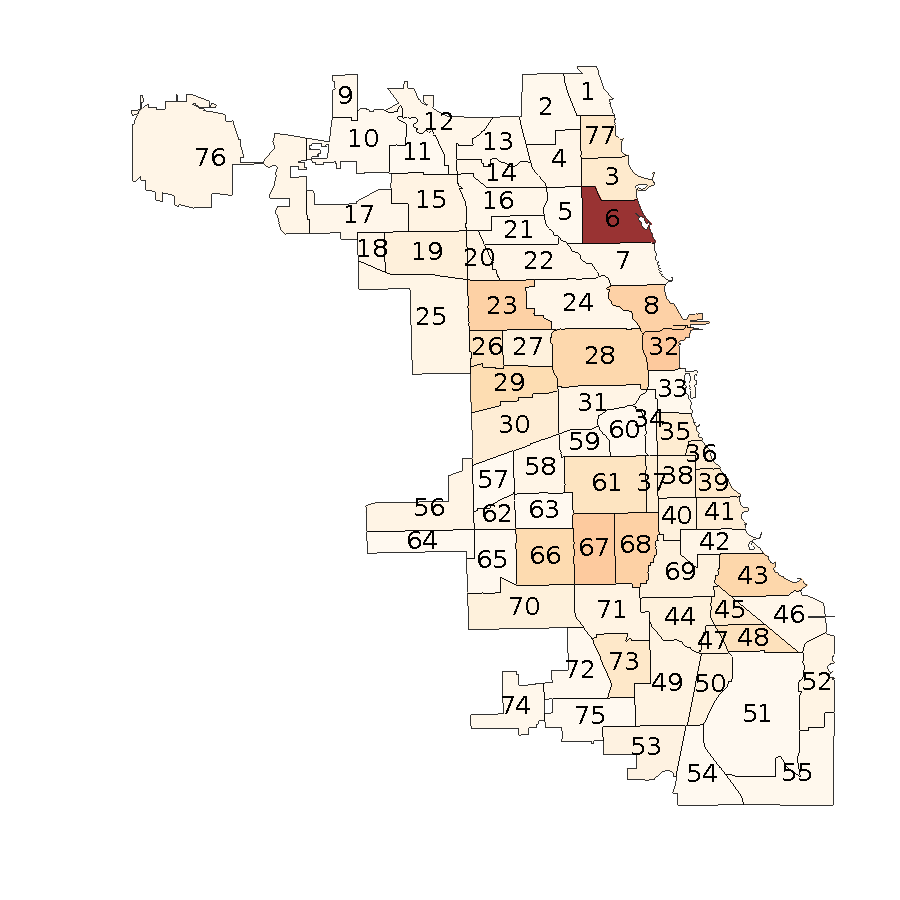
\includegraphics[width=0.4\linewidth]{fig/error_heatmap.pdf}
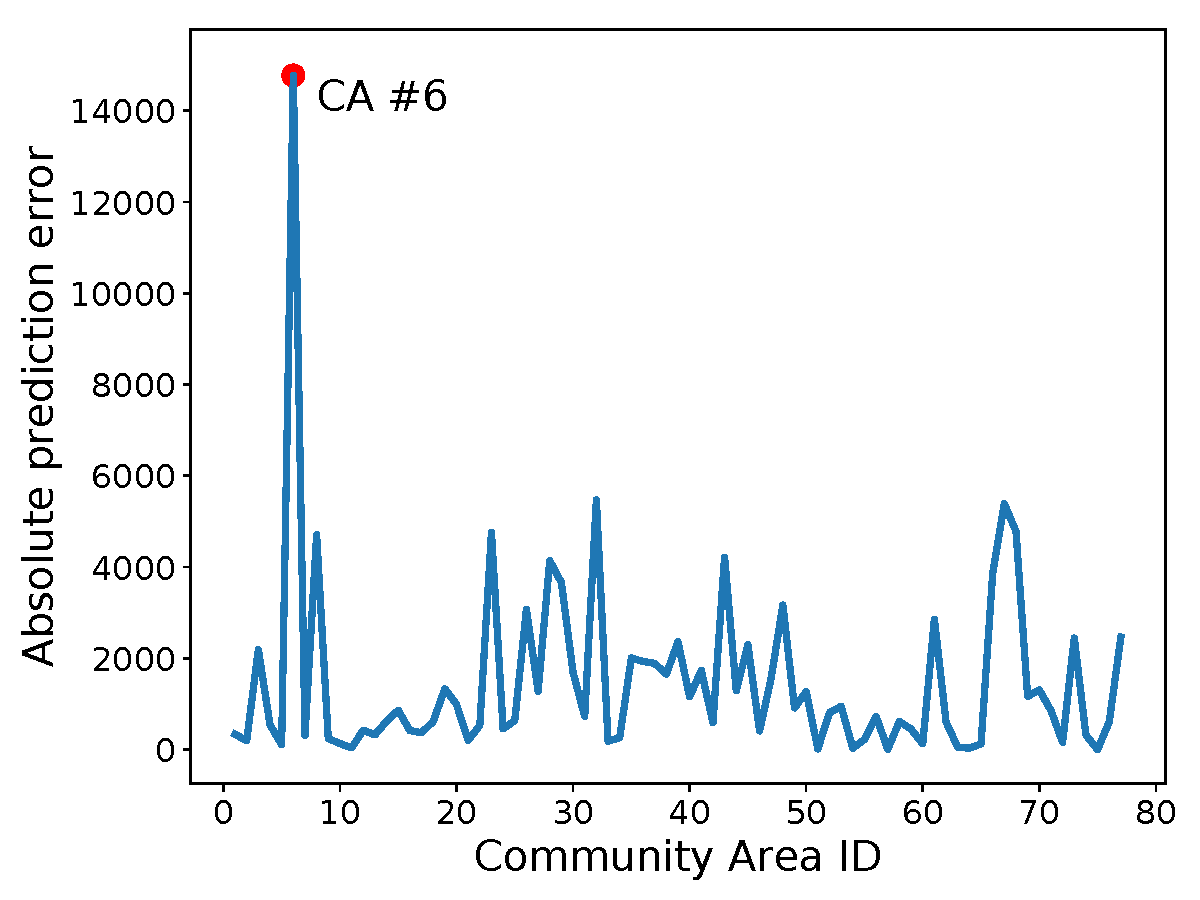
\includegraphics[width=0.5\linewidth]{fig/ca-abs-errors.pdf}
\caption{Crime prediction error at community level in Chicago. The community area \#6 is an outlier with a large error.}
\label{fig:intro}
\end{figure}

\begin{figure}
\centering
\subfigure[Census tracts of community \#6.]{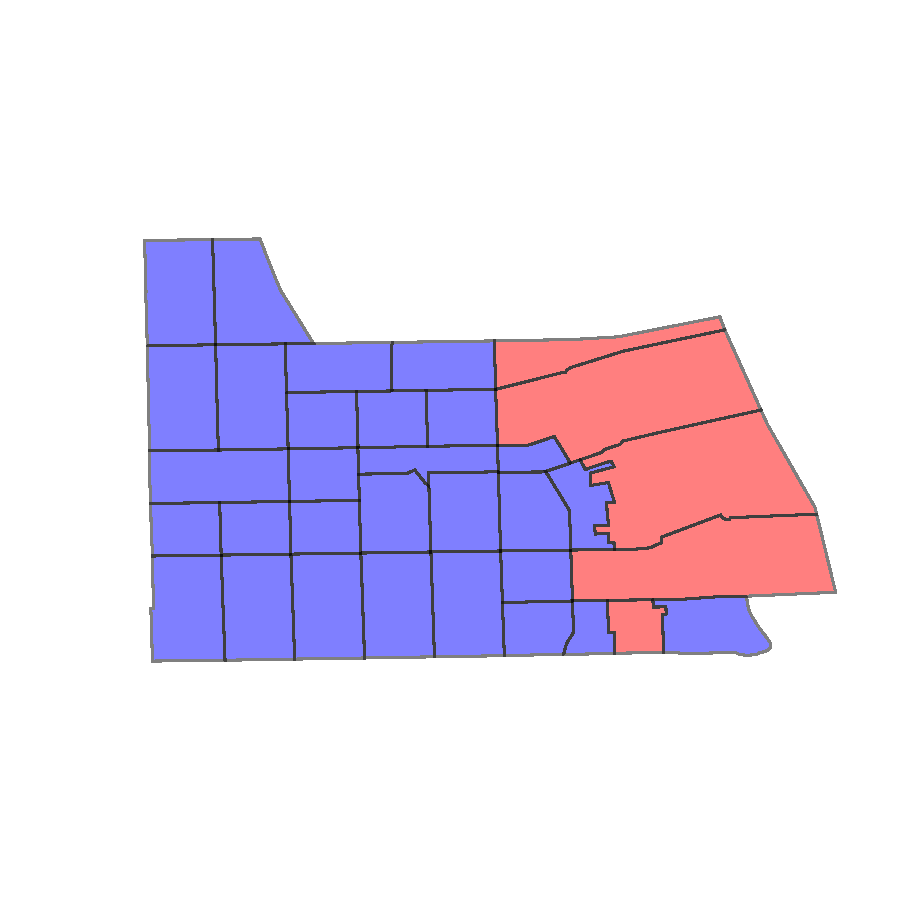
\includegraphics[width=0.5\linewidth]{fig/tracts_within_CA.pdf}}
\subfigure[Tract similarity.]{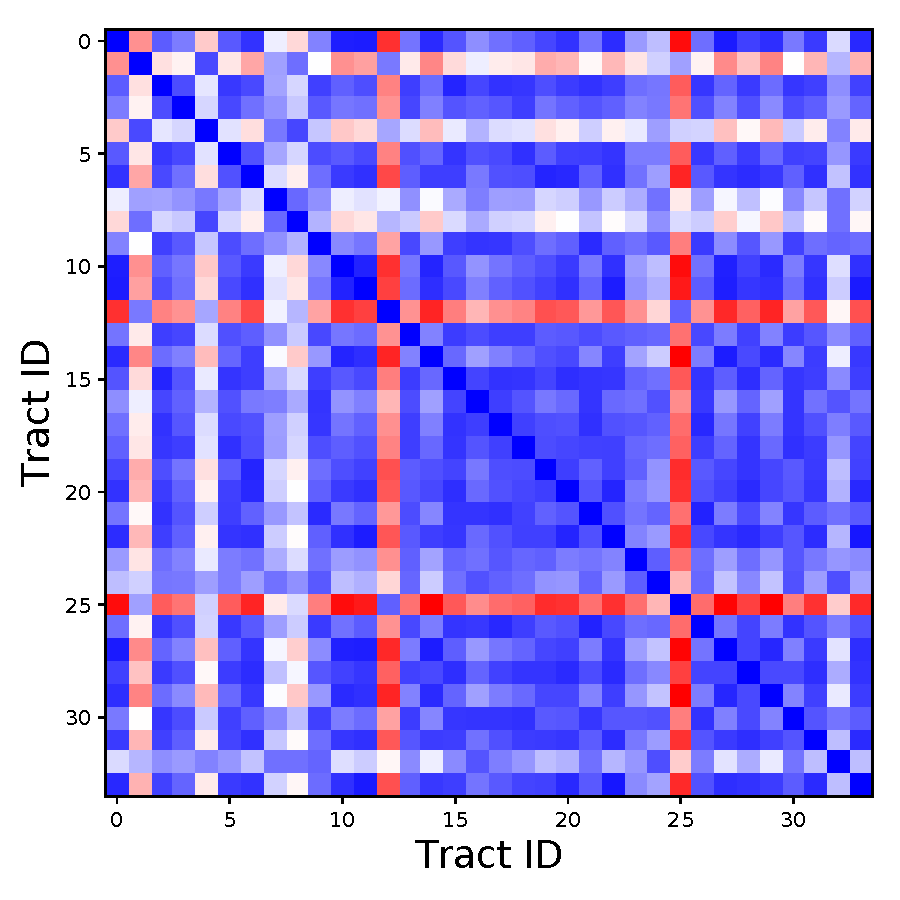
\includegraphics[width=0.45\linewidth]{fig/tract_sim_matrix.pdf}}
\caption{Explaining the outlying community area \#6 in Figure~\ref{fig:intro}. (a) Visualization of the 34 tracts in community \#6. (b) The pair-wise similarity of 34 tracts in terms of demographic feature. It is clear that five tracts (in red color) in the east side are different from other blue tracts.}
\label{fig:intro-explain}
\end{figure}

\begin{example}
We construct a negative binomial model to predict crime count using demographic features by treating each community area as a data sample. Figure~\ref{fig:intro} plots crime prediction error for each community area of Chicago. Community area \#6 (i.e., Lake View area) shows an abnormally high error. In order to explain this outlier, we further investigate the internal structure of this area. Community \#6 consists of 34 census tracts as shown in Figure~\ref{fig:intro-explain}(a).  In Figure~\ref{fig:intro-explain}(b), we visualize the pair-wise Euclidean distance of the demographic features. There are five tracts that are different from other tracts in the demographic feature space, and they all locate in the east side of community \#6. These five tracts, when mixed with other tracts in this community, lead to inferior performance of crime count prediction in that area. 
\end{example}

% problem definition
The observation above motivates us to learn a better region definition for crime study. In this paper, we propose a new problem of \emph{task-specific region partitioning}. Given spatial variables and a pre-defined model (e.g., linear regression), we aim to partition the map into spatial regions such that the model trained by taking regions as data samples achieve the optimal results.

% literature
%two lines of literature: (1) clustering, no target; (2) partition tracts into regions, and build a model for each region.
To the best of our knowledge, task-specific region partitioning is a new problem that has not been studied before. While there exist many methods for spatial clustering~\cite{miller2009geographic}, most of them group the locations based on the similarity of their spatial properties and do not have a target variable to predict. Another similar problem is to partition the locations into $k$ regions and fit a model for each region. Such a problem definition has a different purpose with the goal to show that the correlations between features and target vary over the space (e.g., in some area, disadvantage index  correlates with crime, while in some other areas, it does not). In our problem definition, we aim to fit one model for the whole city hoping to get a generalized interpretation (e.g., disadvantage index  significantly correlates with crime count in Chicago). Such a problem definition is also a more frequently adopted form in criminology literature~\cite{graif2017long}.

% challenge & proposed solution
Task-specific region partitioning is a challenging problem. The key challenge lies in that the region properties (both features and target variable) and the model coefficients change simultaneously when we change the region partition. We prove that it is an NP-hard problem. In our proposed solution, we employ the Markov Chain Monte Carlo (MCMC) method. We start from a pre-defined boundary, and generate a new partition sample by flipping the community area assignment of one tract. Three variants of MCMC methods are proposed to solve this problem. First, a naive MCMC method generates next partition sample by randomly flipping a tract. Second, a heuristic-based MCMC method generates the next sample by flipping one tract randomly selected from the community areas with the highest error. Finally, we employ the reinforcement learning to automatically learn how to generate the next sample that is more likely to improve the prediction performance.


% Experiments results
We evaluate our method on two real datasets, i.e. crime prediction and real estimate price prediction. The learned partitions are shown to consistently outperform the administrative boundaries and spatial clustering method. For example, our method on average outperform administrative boundary by $56\%$ in crime prediction task. We also observe that the heuristic-based MCMC converges faster than the naive MCMC, while the Q-learning MCMC uses the least iterations to converge.

% Key contributions
To summarize, the key contributions of this paper are:
\begin{itemize}[leftmargin=*]
\item We propose a novel problem on task-specific region partitioning. This problem is motivated by real-world urban studies, including our own previous work on crime prediction~\cite{wang2016crime}.
\item We prove the problem is NP-hard and we study different MCMC sampling techniques to solve the problem. 
\item We validate our method through extensive experiments on two real datasets.
\end{itemize}


% Paper organizations
The rest of this paper is organized as follows. Section~\ref{sec:related-work} summarizes related work. The formal definition of our problem is given in Section~\ref{sec:problem}, and our method is described in Section~\ref{sec:method}. Section~\ref{sec:experiment} shows the evaluations on two different tasks. Finally, we conclude in Section~\ref{sec:conclusion}.

